% This file was created by matplotlib2tikz v0.7.3.
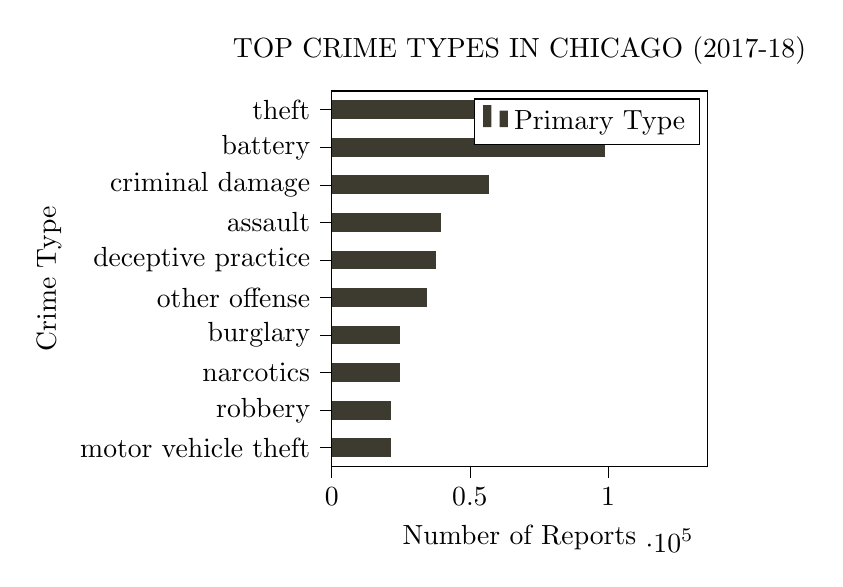
\begin{tikzpicture}

\definecolor{color0}{rgb}{0.23921568627451,0.231372549019608,0.188235294117647}

\begin{axis}[
height=2.5in,
tick align=outside,
tick pos=left,
title={\printsubsection{\MakeUppercase{Top Crime Types in Chicago (2017-18)}}},
width=2.5in,
x grid style={white!69.01960784313725!black},
xlabel={Number of Reports},
xmin=0, xmax=135895.2,
xtick style={color=black},
y grid style={white!69.01960784313725!black},
ylabel={Crime Type},
ymin=-0.5, ymax=9.5,
ytick style={color=black},
ytick={0,1,2,3,4,5,6,7,8,9},
yticklabels={motor vehicle theft,robbery,narcotics,burglary,other offense,deceptive practice,assault,criminal damage,battery,theft}
]
\draw[fill=color0,draw opacity=0] (axis cs:0,-0.25) rectangle (axis cs:21393,0.25);
\addlegendimage{ybar,ybar legend,fill=color0,draw opacity=0};
\addlegendentry{Primary Type}

\draw[fill=color0,draw opacity=0] (axis cs:0,0.75) rectangle (axis cs:21560,1.25);
\draw[fill=color0,draw opacity=0] (axis cs:0,1.75) rectangle (axis cs:24645,2.25);
\draw[fill=color0,draw opacity=0] (axis cs:0,2.75) rectangle (axis cs:24730,3.25);
\draw[fill=color0,draw opacity=0] (axis cs:0,3.75) rectangle (axis cs:34352,4.25);
\draw[fill=color0,draw opacity=0] (axis cs:0,4.75) rectangle (axis cs:37741,5.25);
\draw[fill=color0,draw opacity=0] (axis cs:0,5.75) rectangle (axis cs:39680,6.25);
\draw[fill=color0,draw opacity=0] (axis cs:0,6.75) rectangle (axis cs:56848,7.25);
\draw[fill=color0,draw opacity=0] (axis cs:0,7.75) rectangle (axis cs:98995,8.25);
\draw[fill=color0,draw opacity=0] (axis cs:0,8.75) rectangle (axis cs:129424,9.25);
\end{axis}

\end{tikzpicture}